\subsection{Power Subsystem}
\label{sec:power_subsystem}
The power system is an important part to any electrical device or component that requires any amount of power. Most often, it starts from a power source such as a battery or wall outlet then is converted into energy to operate what is being used. At the minimum, this model is designed to be an independent system, having the capability to operate on its own. The way that can be achieved is through solar power. \par
Solar power has been such a strong growing source of energy and will play a vital role in our system. Power is collected through the solar panels and then regulated through the charge controller to ensure that the battery is receiving the correct amount of charge. The power is regulated through the charge controller so that the battery is not being over charge, which could potentially damage it and reduce the battery life in the future. It is then stored in a battery when the system is not operating and then utilized when needed. From there, voltage needs to be regulated again throught the voltage regulator for the microcontroller and other components that require different amounts of voltage. The block diagram in \autoref{fig:power-block-diagram} shows the flow of power through the system. 

\begin{figure}[H]
    \centering
    \caption{Power subsystem block diagram}
    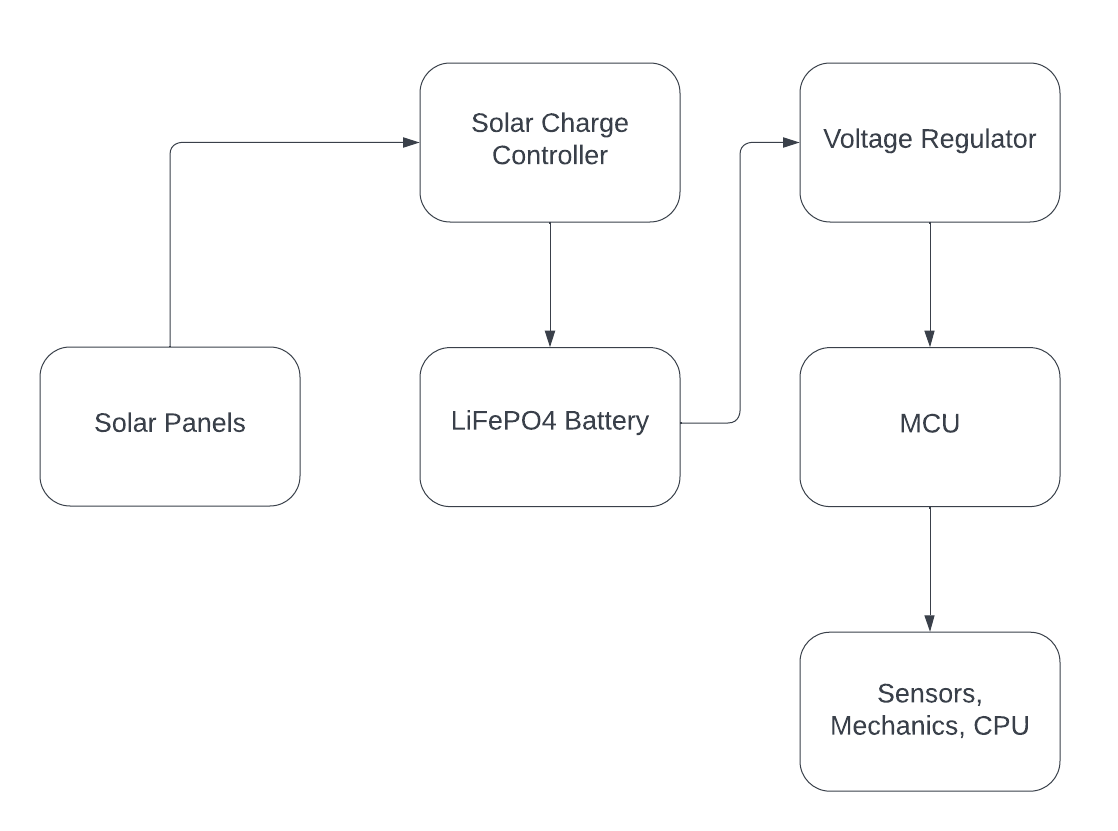
\includegraphics[width=\textwidth]{images/Power_System_Flowchart.png}
    \label{fig:power-block-diagram}
\end{figure}
The block labeled ``Mechanics'' in \autoref{fig:power-block-diagram} refers to the solenoid valve for controlling water flow as well as the control scheme for actuating the solar panels to maximize power efficiency.
\subsubsection{Solar Panel Control}
To get a greater degree of accuracy the use of stepper motors are used. First, based on the choice of solar panels we get the mass and dimensions of the solar panels, these are .76kg and .336m x .2m respectively. This is important for calculating the torque. We only need to provide two degrees of freedom, one about the short axis (the horizontal axis that bisects the .2m side) and the vertical axis (the axis at the intersection that bisects the two sides of the panel). From the length and mass we can calculate the force per unit length:
\begin{equation}
    \frac{.76 \text{kg}}{.336 \text{m}}=22.62\frac{\text{N}}{\text{m}}
    \label{eqn:short-axis-fpl}
\end{equation}
Now, knowing that torque is $F\times d$ we can formulate the torque for any given angle about this axis in the following:
\begin{equation}
    \int_{0}^{.168} 22.62 \times x \times \sin{\theta} \, dx
    \label{eqn:short-axis-torque}
\end{equation}
\autoref{eqn:short-axis-torque} gives the torque for any given angle. Something you might have noticed is that this is for only one side of the panel. The full torque about the central axis is as follows:
\begin{equation}
    \int_{0}^{.168} 22.62 \times x \times \sin{\theta} \, dx - \int_{0}^{.168} 22.62 \times x \times \sin{180-\theta} \, dx
    \label{eqn:short-axis-torque-total}
\end{equation}
From \autoref{eqn:short-axis-torque-total} we can find the maximum and minimum values of the torque about the axis by finding the crossings of the first derivative with respect to $\theta$ and finding the concavity in the second derivate with respect to $\theta$. Doing so proves the intuition that there is no torque around either axis, this equation evaluates to 0 for all $\theta$.

To save on power \autoref{fig:stepper-config} shows that two motors will work to rotate the panels about the short axis while the center axis is actuated by a single motor and belt system.
\begin{figure}[H]
    \centering
    \caption{Stepper motor configuration}
    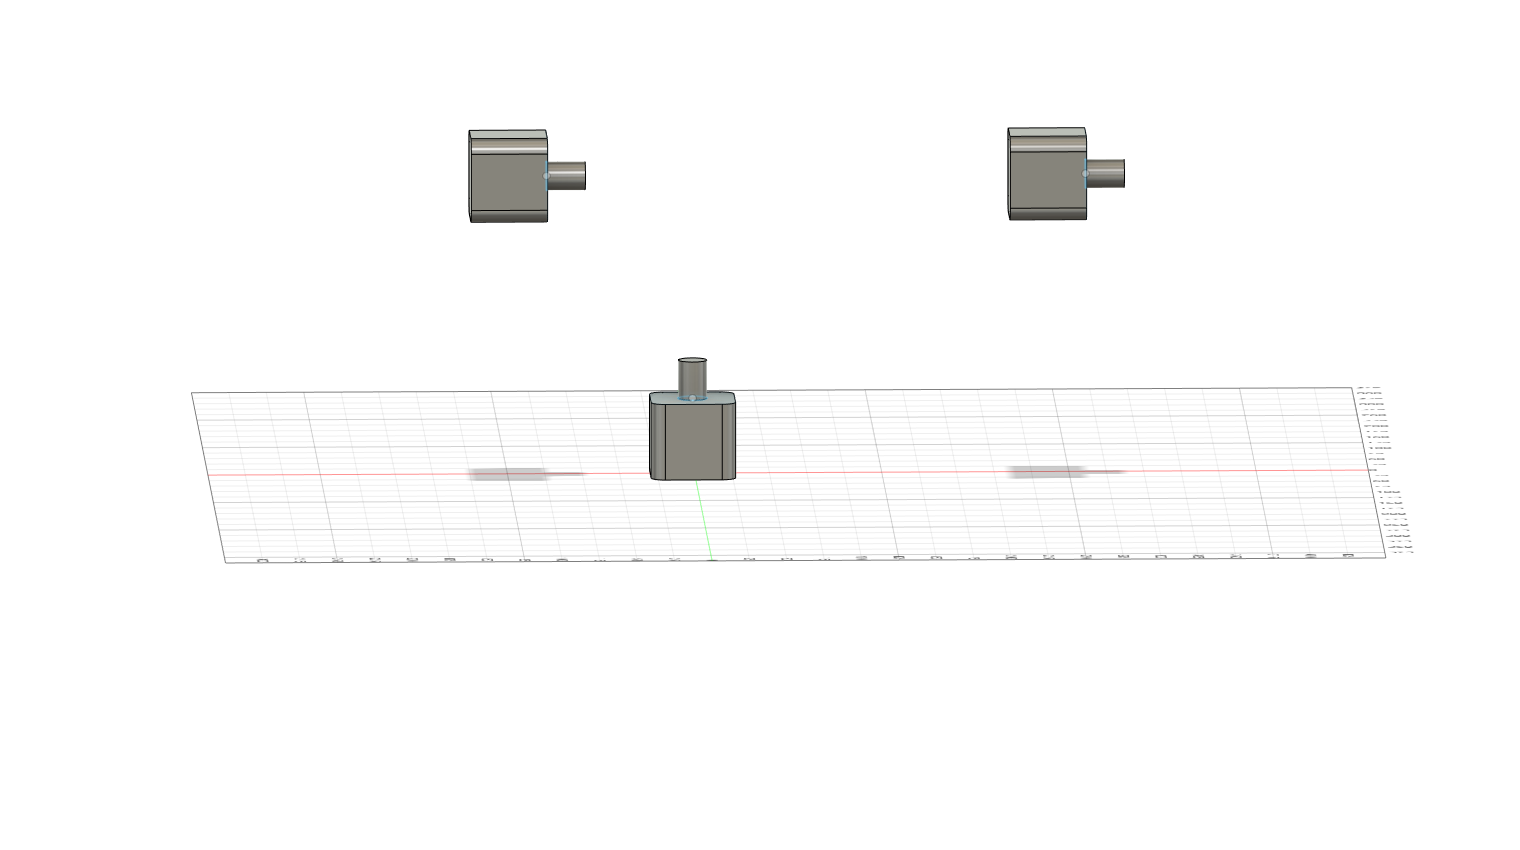
\includegraphics[width=0.5\textwidth]{images/stepper-config.png}
    \label{fig:stepper-config}
\end{figure}
The reason we have to use two stepper motors for the short axis rotation is that because as the panels rotate about their central axis any rod or pulley or tensioner system would come out of alignment. Another advantage of this due to the lack of torque in the system is that using a motor controller the two motors can be driven with a single H-bridge with a minimum penalty to power, this will ensure that both panels are always pointed at the same angle in the desired direction.\par
\subsubsection{Voltage Regulator Designs}
As mentioned before, voltage regulators play an important role in regulating voltage throughout the whole model. They make sure that all the components like the microcontroller, sensors, mechanics, etc. are receiving the right amount of voltage.\par
The CC3220 requires 3.3V to operate and the sensors will be running on 5V. With the battery running at 12V, we would use the voltage regulator to supply the right voltage amount to each component. To perform and achieve the proper regulation, we created different design schematics for the LM317 (Linear) voltage regulator and the LM2576 (Switching) regulator. Along with that, we created DC/DC designs on WEBENCH as a consideration for specific conditions.\par
\paragraph{Linear Voltage Regulator Designs}
The linear voltage regulator schematic was designed to generate an output voltage of 3.3V for the CC3220. This circuit schematic is obtained from the LM317 voltage regulator datasheet, Figure 39, and then designed on Multisim with capacitors, resistors, and diodes. From the datasheet, there were values that were given and from there we had to find values and then test them. The CADJ we used 1uF as a constant and then 390Ω was used for the value R. With these inputed values, we achieved an estimated 3.3V and measuring the adjustment current we got 5.2634mA as shown in Figure 40.\par
\begin{figure}[H]
    \centering
    \caption{LM317 Linear Voltage Regulator }
    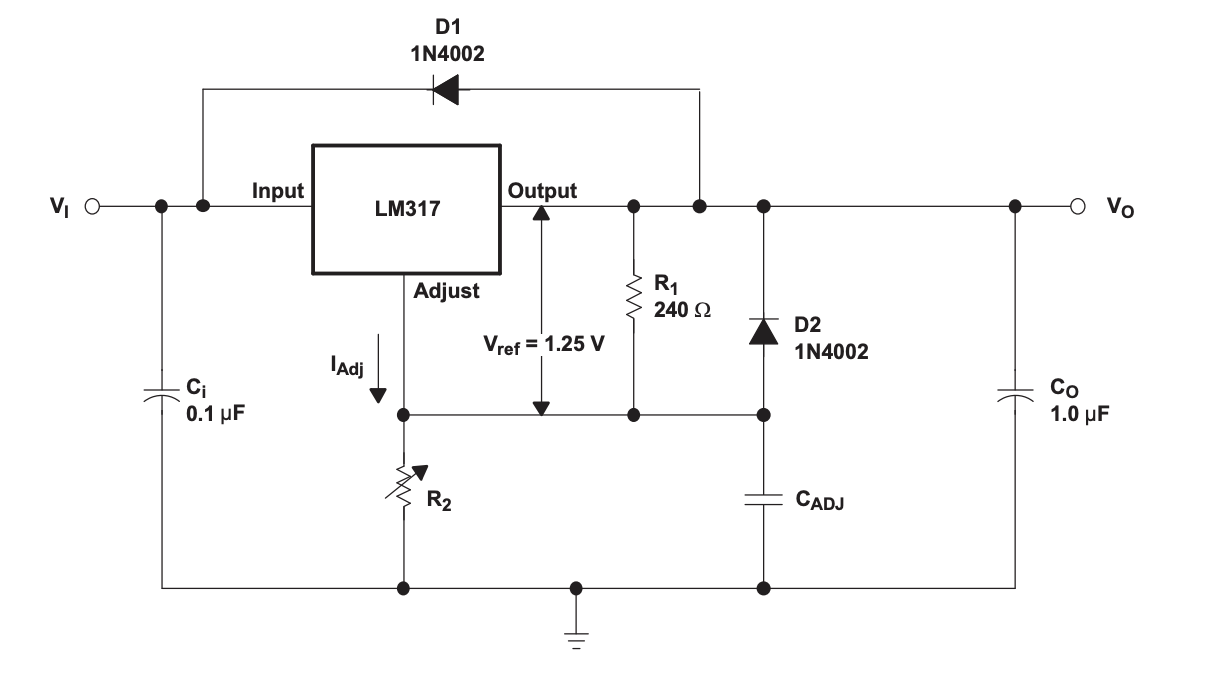
\includegraphics[width=\textwidth]{images/LM317_Application_schematic.png}
    \label{fig:linear-voltage-regulator}
\end{figure}
\begin{figure}[H]
    \centering
    \caption{LM317 3.3V Linear Voltage Regulator}
    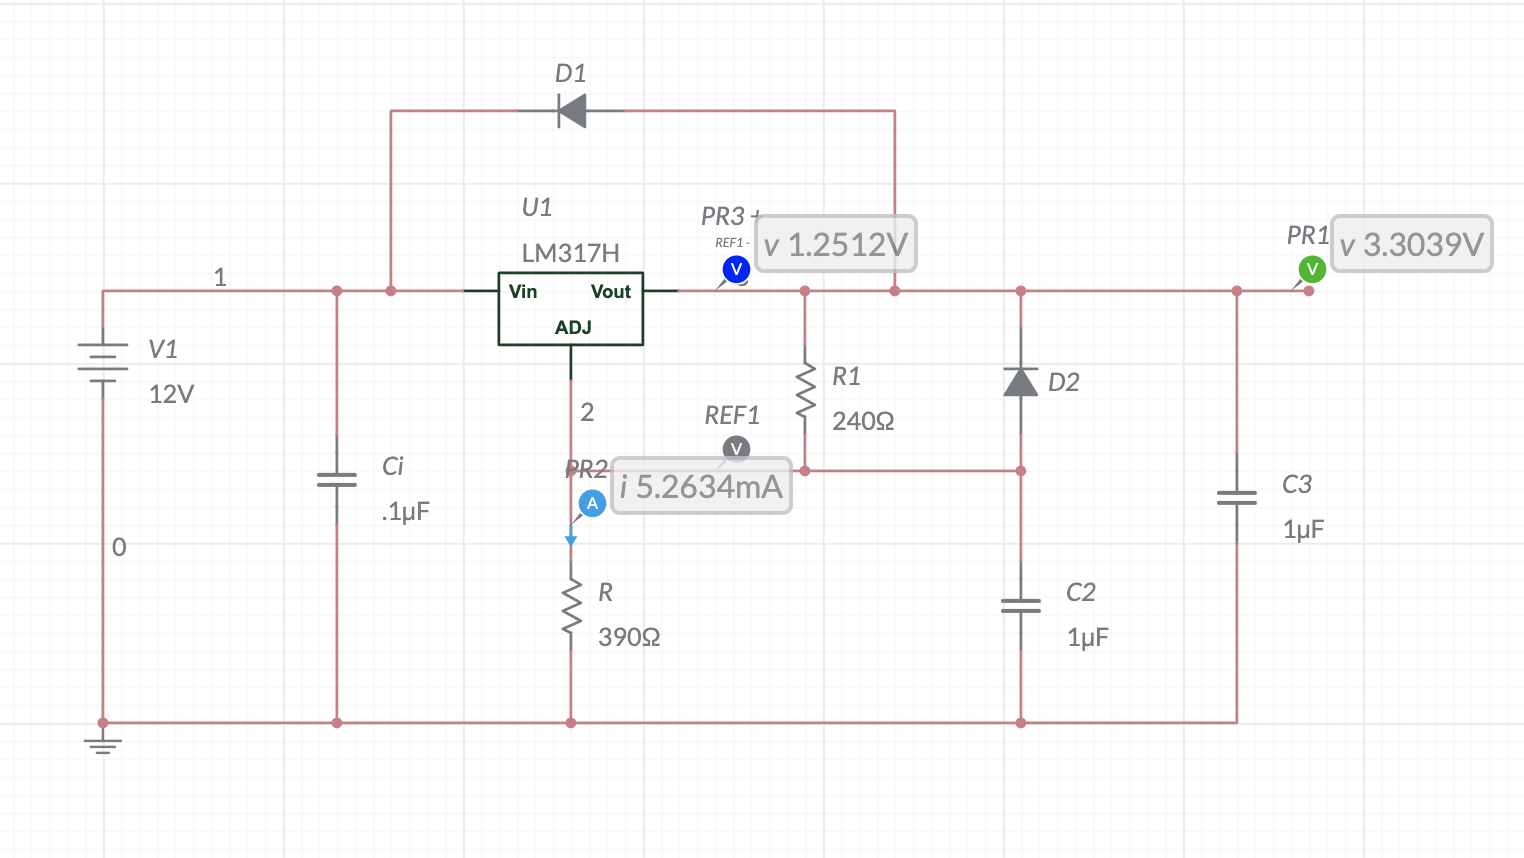
\includegraphics[width=\textwidth]{images/LM317_3_3_schematic.png}
    \label{fig:3.3V-linear-voltage-regulator}
\end{figure}
In Figure 41, we re-designed the ciruit get the regulated output voltage of approximately 5V for the sensors. This is done with the same circuit as for the 3.3 output voltage regulation, but the value R is now 720Ω with CADJ still remaining at 1uF. With these values that we found we achieved an output voltage of about 5V and the adjustment current of 5.2617mA.\par
\begin{figure}[H]
    \centering
    \caption{LM317 5V Linear Voltage Regulator}
    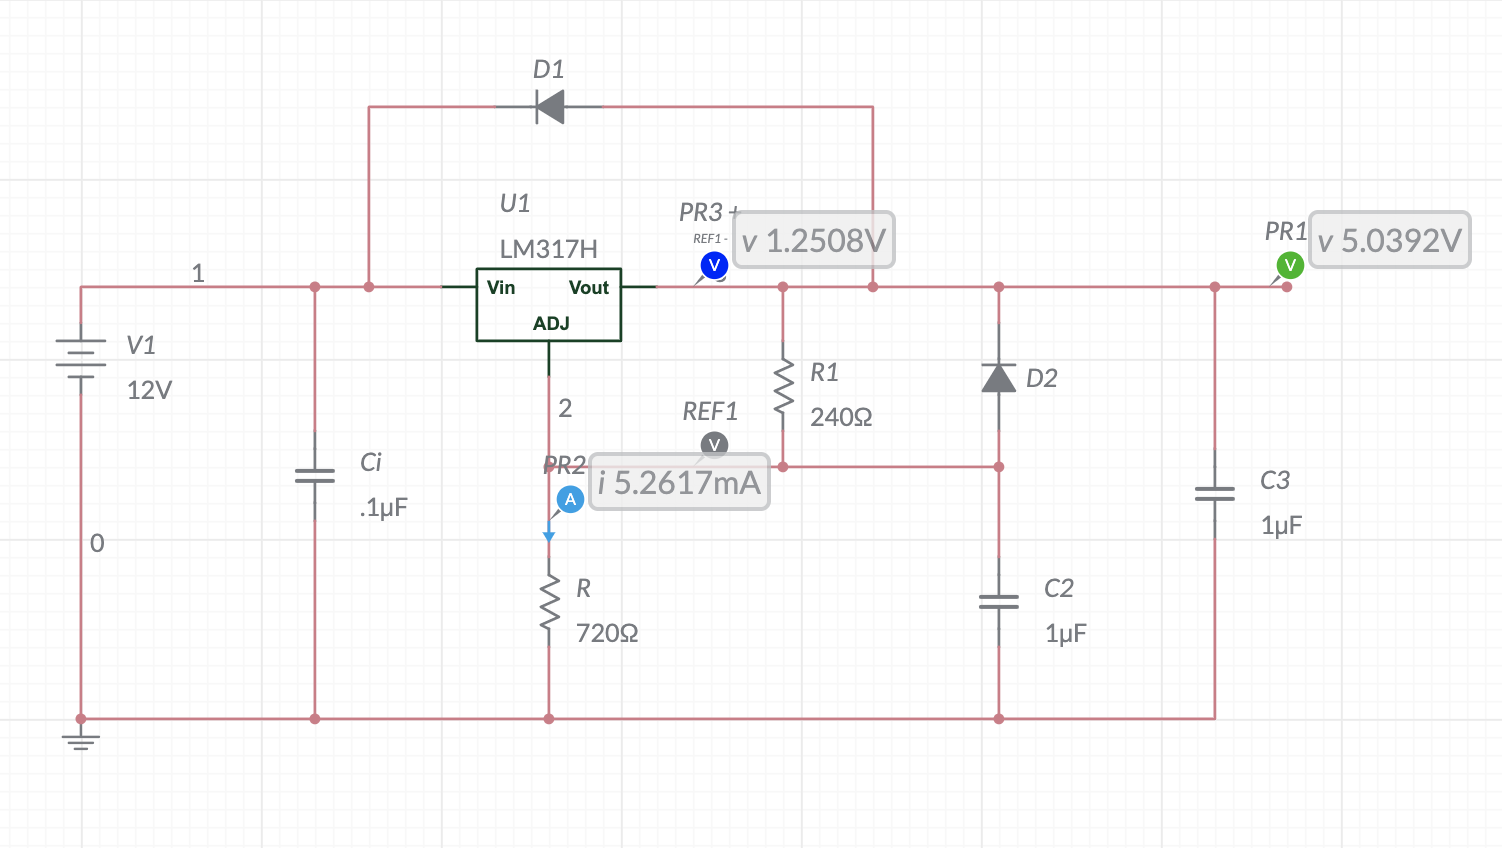
\includegraphics[width=\textwidth]{images/LM317_5_schematic.png}
    \label{fig:5V-linear-voltage-regulator}
\end{figure}
\paragraph{}In this testing, we were able to verify that the LM317 Linear voltage regulator can output the proper voltages. Along with this testing, we also went ahead to see if the voltage regulator was able to output higher voltage levels. For this testing we wanted to see if we could achieve a regulated output voltage of 12V. Using the same circuit for the output voltages 3.3V and 5V, we changed the value of R to increase the output voltage. We were unable to get the regulated 12V from the output. Instead, the highest that it went up to was about less than 11V. During this test though, we noticed that when we past 2kΩ the adjusttment current and the voltage reference started to decrease. Not only that but the output voltage stayed between 10V and 11V, but didn't go higher than 11V.
\begin{figure}[H]
    \centering
    \caption{LM317 10V Linear Voltage Regulator}
    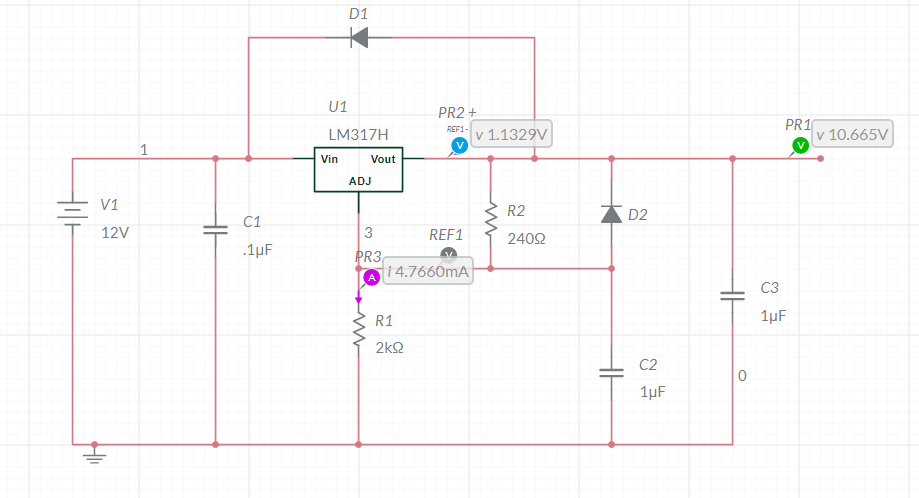
\includegraphics[width=\textwidth]{images/LM317_10_schematic.png}
    \label{fig:10V-linear-voltage-regulator}
\end{figure}
\paragraph{Switching Voltage Regulator Designs}
The same approach was used for the switching voltage regulator to find out how to achieve the correct output voltage. This will be done for the CC3220 microcontroller that operates at 3.3V and the sensors operating at 5V. Luckily, in the Texas Instrument datasheet they had 2 different versions of their schematic done for their fixed version as well as their adjustable version. In the fixed version, we are able to set the output regulated voltages to different levels, such as 3.3, 5, 12, and 15V, leaving the load current fixed to 3A. This is shown in the figure below.\par
\begin{figure}[H]
    \centering
    \caption{LM2576 Fixed Switching Voltage Regulator}
    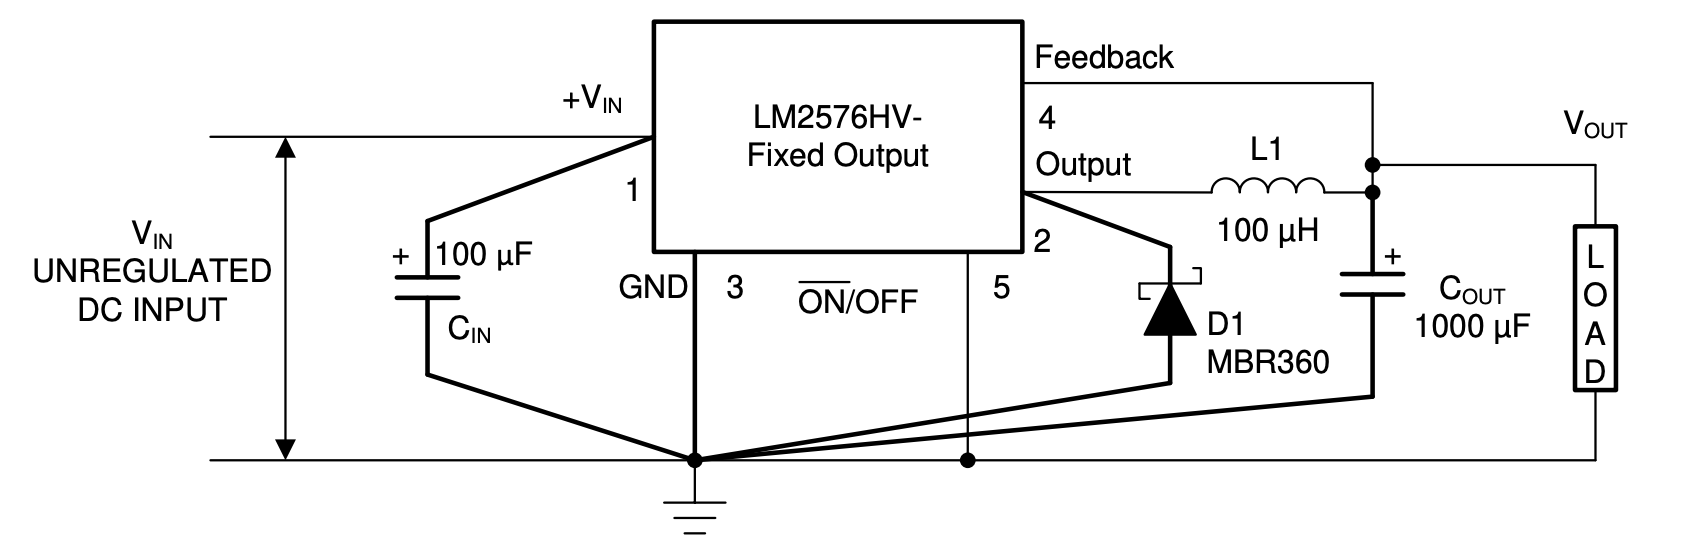
\includegraphics[width=\textwidth]{images/LM2576_Fixed.png}
    \label{fig:fixed-switching-voltage-regulator}
\end{figure}
For the adjustable version of the LM2576 switching voltage regulator, because it is adjustable, the maximum input voltage that is allowed by this version is 25V. The output regulated voltage can also only output 10V, maximum, with a constant load current of 3A, similar to the fixed version. This is shown in Figure 42. In this version as well we can see that values R1 and R2, on the right, need to be found to find the Vout. This can be done with the equations below as well.\par
\begin{figure}[H]
    \centering
    \caption{LM317 adjustable switching Voltage Regulator}
    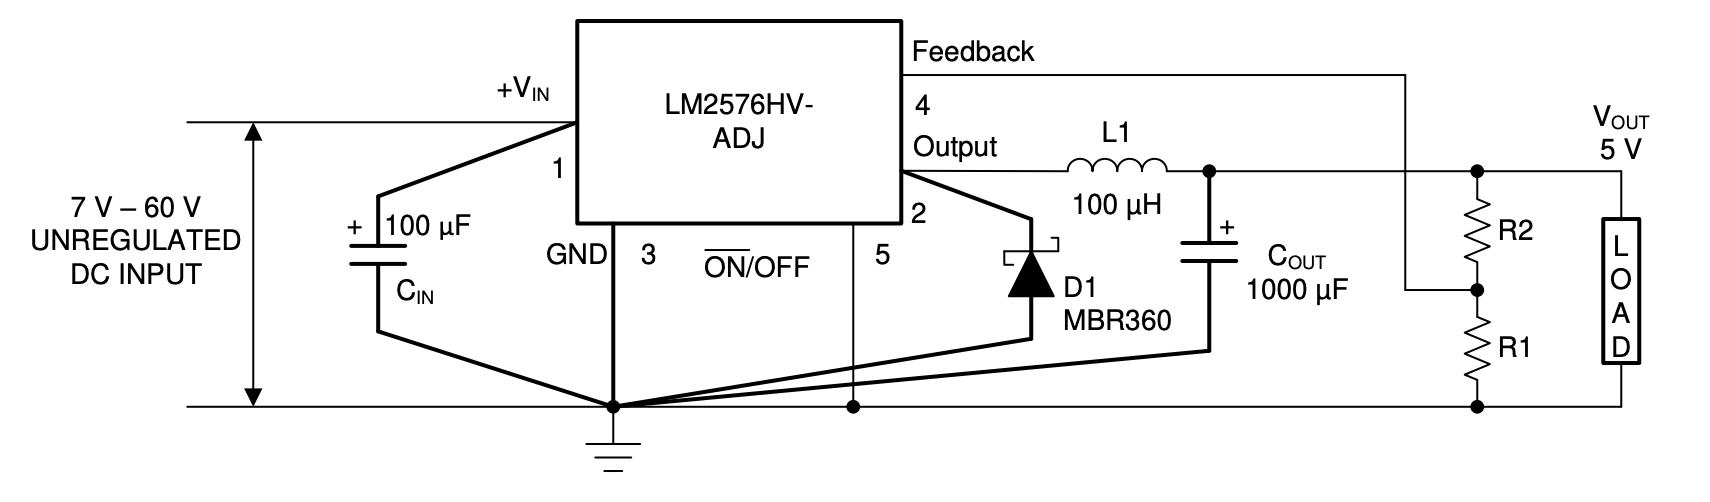
\includegraphics[width=\textwidth]{images/LM2576_Adjustable.png}
    \label{fig:adj-switching-voltage-regulator}
\end{figure}

\begin{figure}[H]
    \centering
    \caption{Switching Voltage Regulator Equations}
    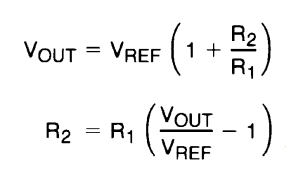
\includegraphics[width=\textwidth]{images/LM2576_Adjustable_equations.png}
    \label{fig:switching-voltage-regulator-equations}
\end{figure}
For this adjustable version, there is obviously no fixed value that the output voltage has to be. In this case, let's say the minimum outpute voltage of 10V We would still need to find the value in for 4 and the regulator chosen for. \par
We were also able to find this specific switching voltage regulator on WEBENCH as well, in the figure below. Reading what was on WEBENCH this specific design is able to provide, 86\% efficiency, has a BOM cost of \$9.84, and has a footprint of $957mm^2$. In this circuit design, to achieve the correct regulated output voltage, it is all dependant on the values Rfbt and Rfbb. This gives the ideal resistances that allows the circuit to reach the right voltages. Luckily, were able to find this design on WEBENCH, because it helps have a better understanding for this voltage regulator with the cost and efficiency that it provides. 
\begin{figure}[H]
    \centering
    \caption{LM2576 WEBENCH Design}
    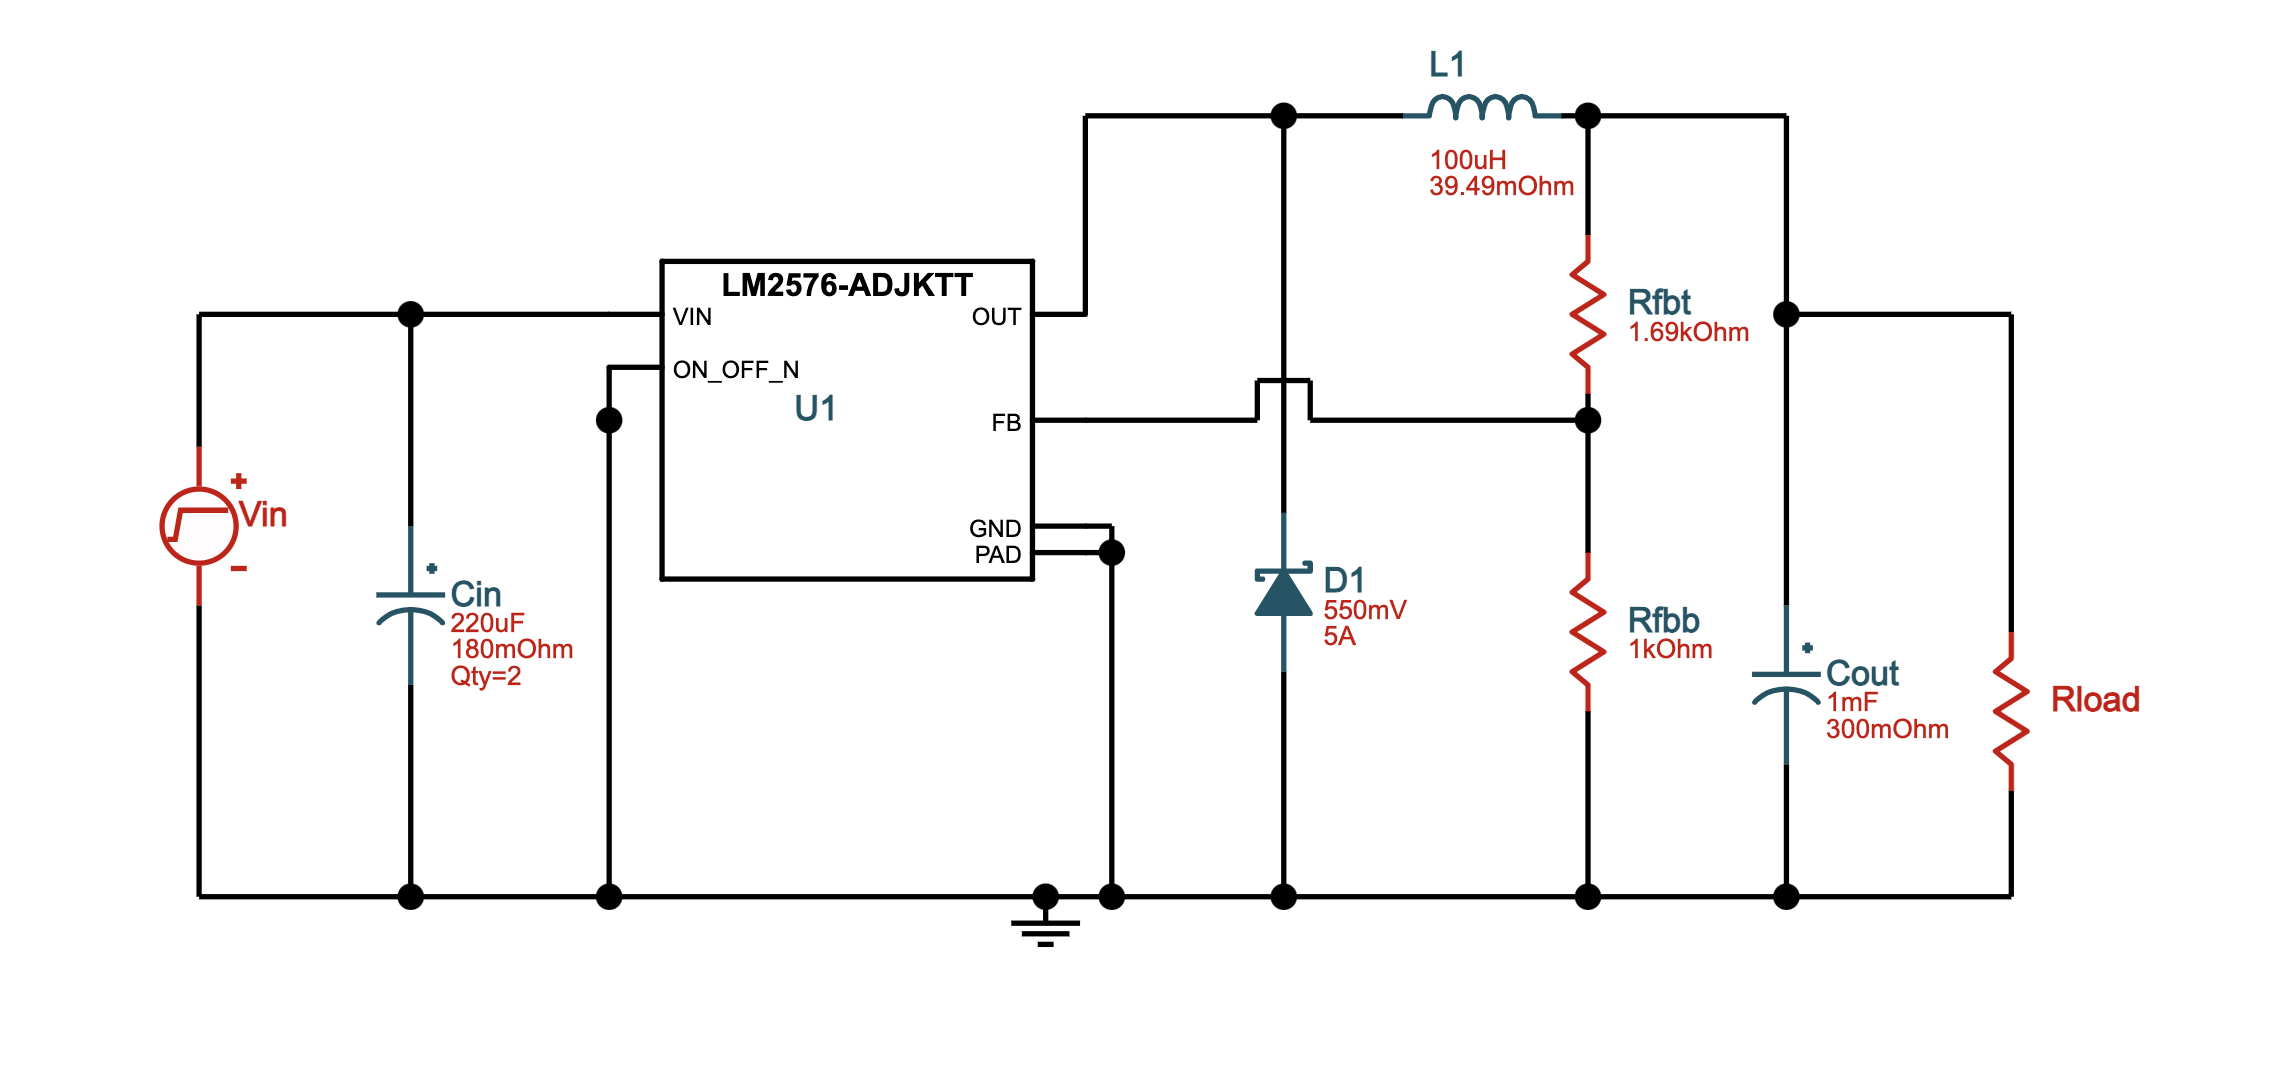
\includegraphics[width=\textwidth]{images/LM2576_WEBENCH.png}
    \label{fig:LM2576 WEBENCH Design}
\end{figure}
\paragraph{WEBENCH Designs}
 WEBENCH is a resource by Texas Instruments that helps design power supplies easily. This resource can be used for DC/DC power systems and AC/DC power systems. It is customizable and helps create various power supply circuits. In this software, we have the freedom to pick and choose our input and output values, and also consider if we want the desired circuit to be balanced, low cost, have high efficiency, or have a small footprint. \par
 For this system, we used input values between 8V and 22V and then output values of 3.3V with max current of 3A. With this we were able to find TPS62933, a high-efficiency, wide input range buck converter that is easy to use. This design itself provides an efficiency of 86.5\%, a BOM cost of \$1.34, and footprint of $195mm^2$. This is one of their low cost designs.\par
 \begin{figure}[H]
    \centering
    \caption{TPS62933}
    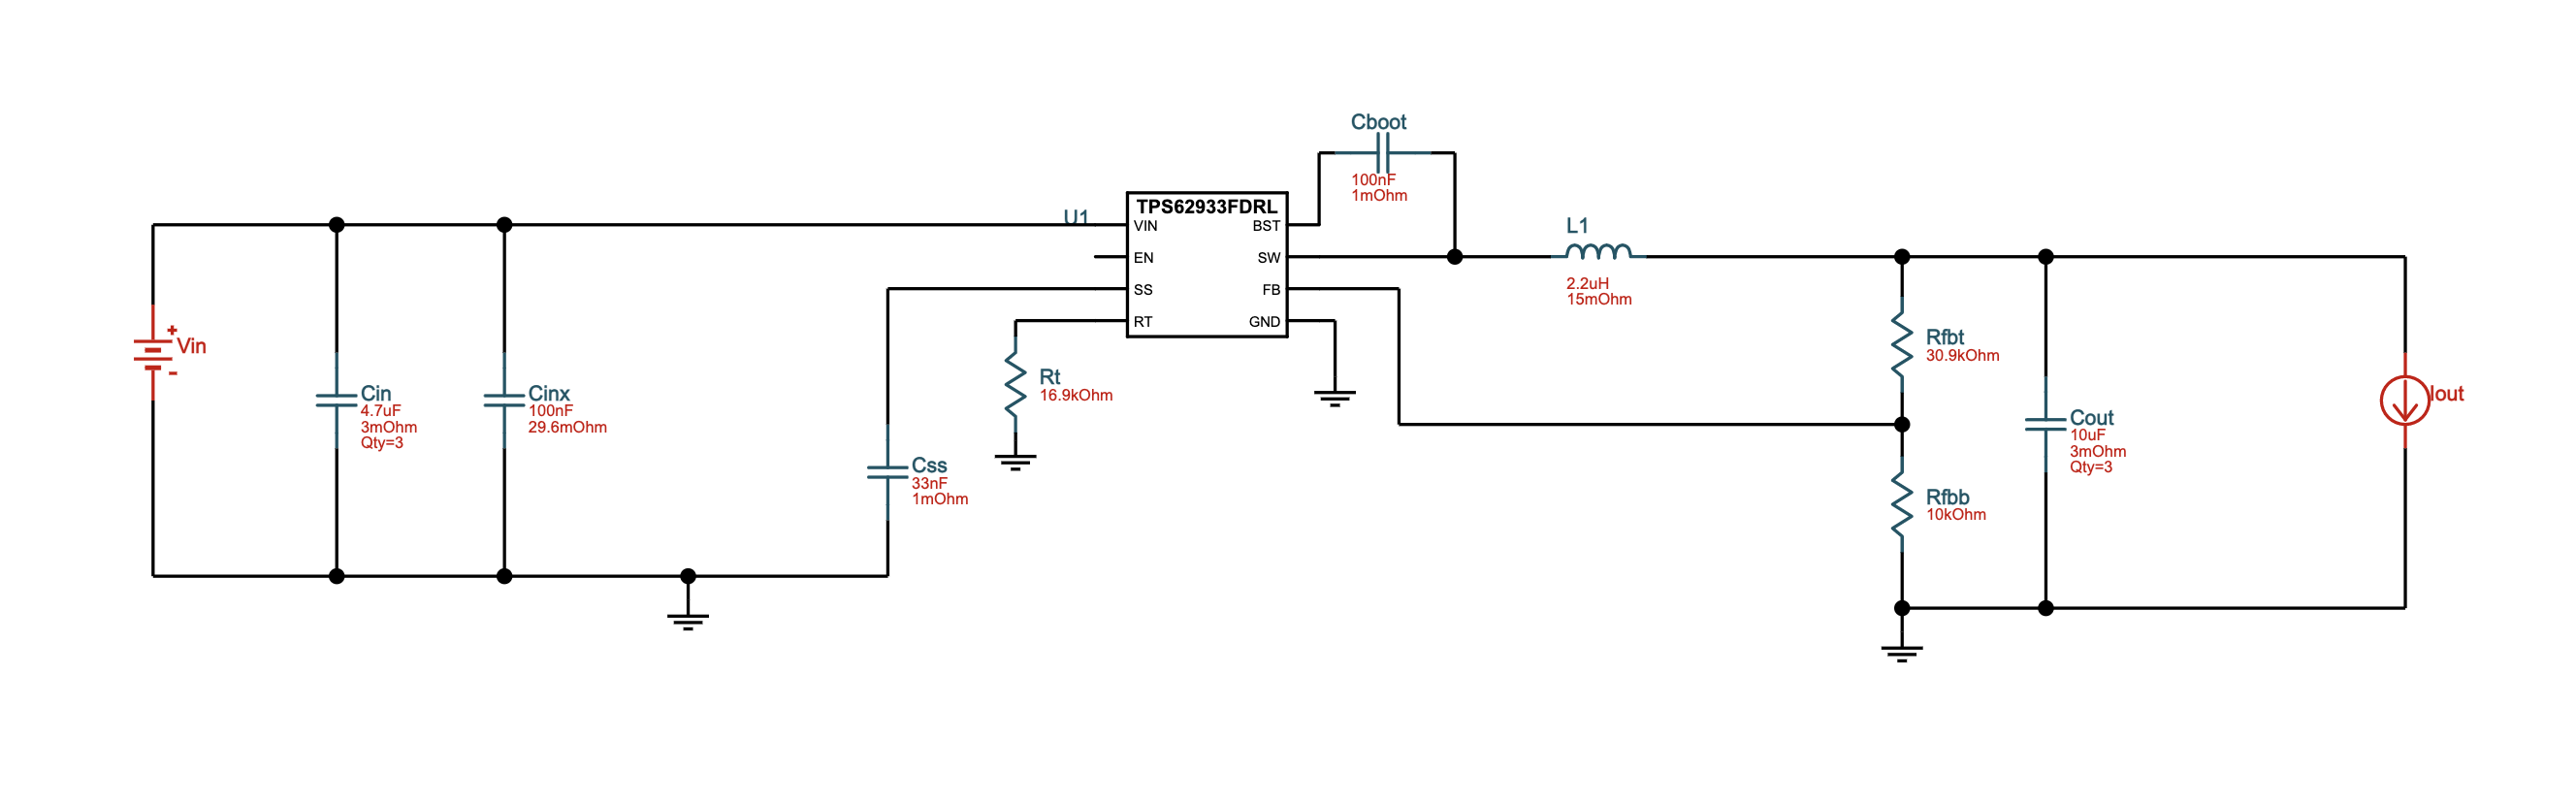
\includegraphics[width=\textwidth]{images/TPS62933.png}
    \label{fig:WEBENCH Design TPS62933}
\end{figure}
For the output regulated voltage 5V, the TPS62933 is also compatible for the 5V output regulation. Going back and changing the output value to 5V and changing the desired circuit consideration to a balanced circuit we find the TPS563300. This is also a high-efficient, easy-to-use buck converter that has a wide input range of 3.8V to 28V, but also supports an output current of 3A and regulates .8V up to 22V. The TPS563300 provides an efficiency of 91.5\%, a BOM of \$1.42, but a footprint of $516mm^2$. \par
\begin{figure}[H]
    \centering
    \caption{TPS563300}
    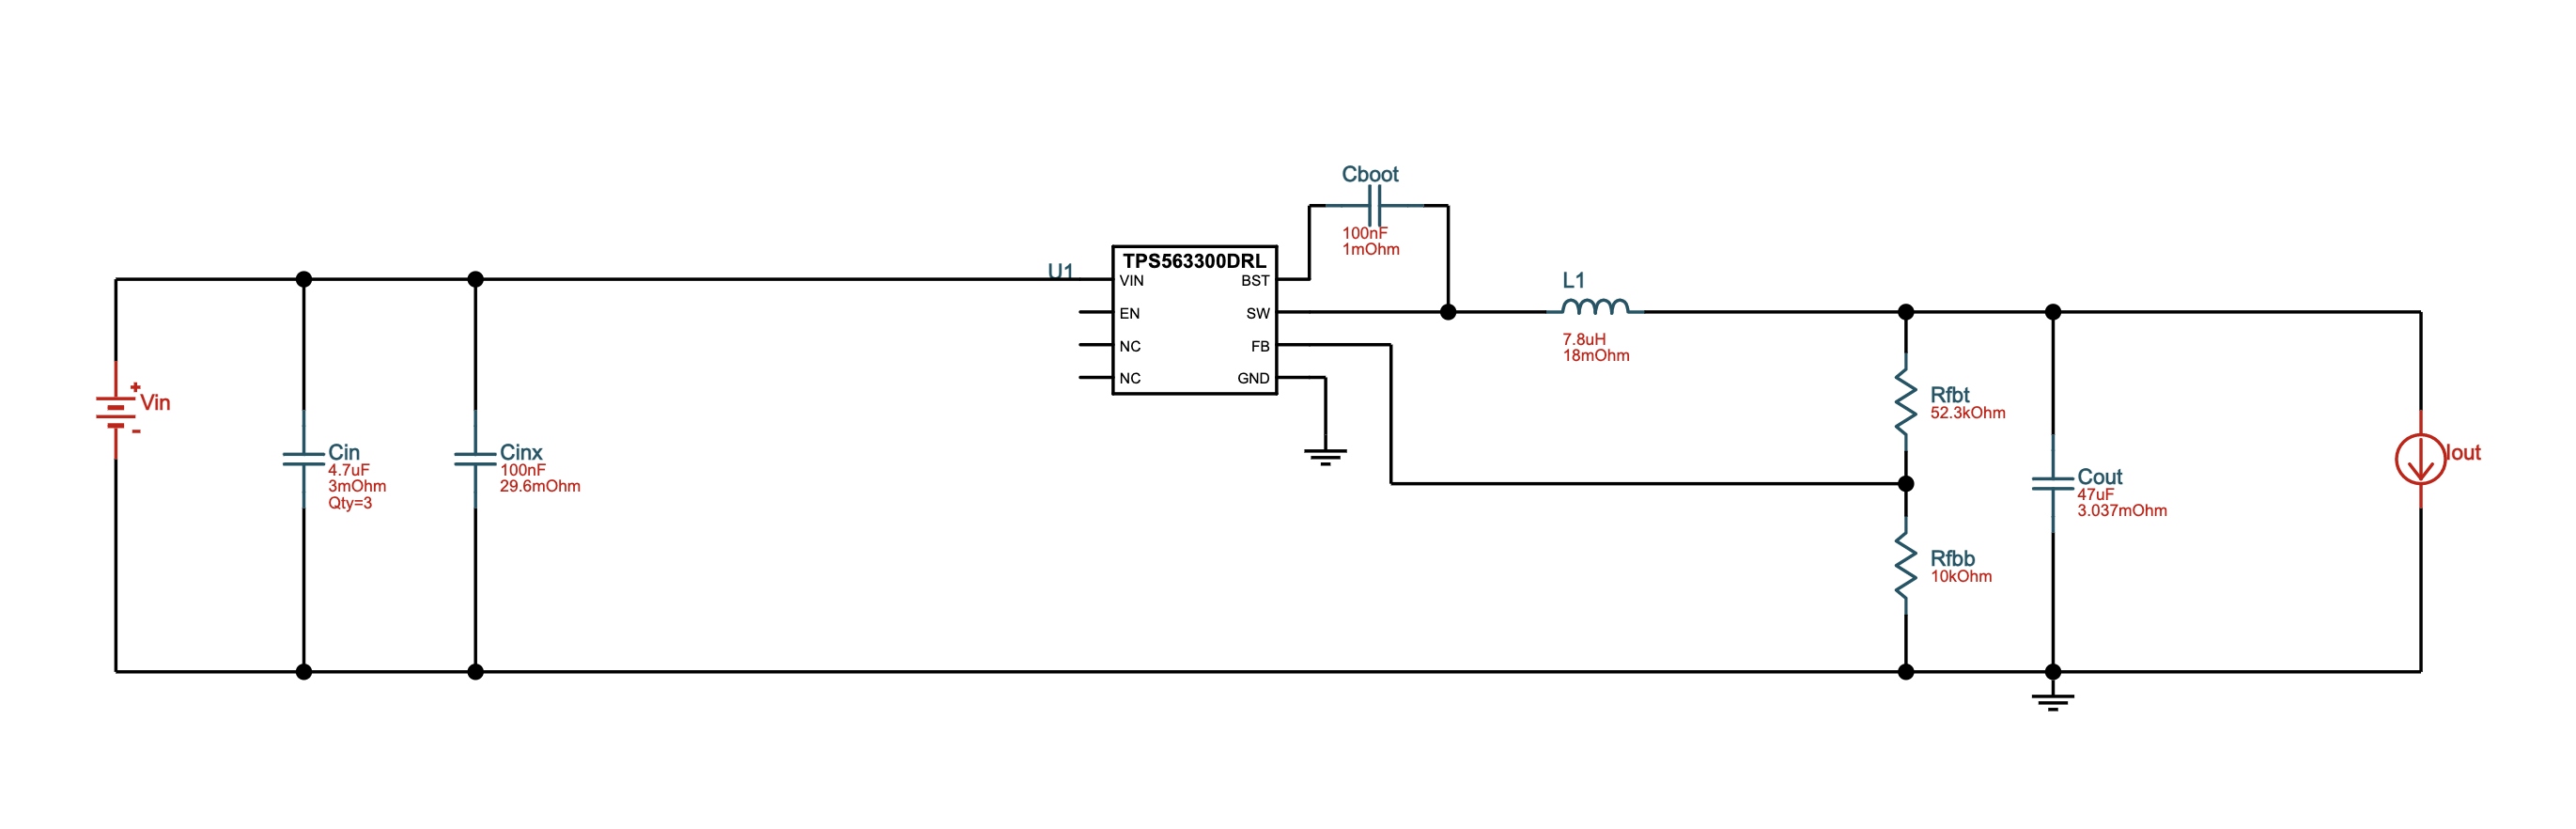
\includegraphics[width=\textwidth]{images/TPS563300.png}
    \label{fig:WEBENCH Design TPS563300}
\end{figure}
Although the TPS563300 is bigger, the price for the high efficiency this design provided would have been very good. It also doesn’t have that many other electrical components compared to the TPS62933, which adds to why it is easy-to-use.\par
After we are able to get all of the parts and components for the designed voltage regulators circuits, we can start testing each of them to see if the regulators are giving the proper output voltage and current that we theoretically found.\par